\chapter{Resultados e Discussão}\label{cap:resultados}

\section{Sequenciamento e controle de qualidade das leituras}
Após o sequenciamento das amostras, foram obtidas 7.8 milhões de leituras de tamanho médio de 
223 pares de base para a amostra ACT016 e 7.4 milhões de leituras com tamanho médio de 222 pares de base
para a amostra ACT094. Após a filtrar as leituras utilizando a ferramenta Trimmomatic, retivemos
6.2 milhões de leituras com tamanho médio 113 pares de base \(perda 21,5\%\) para ACT016 e 6.1 milhões
de leituras com tamanho médio 145 pares de base\(perda de 18,5\%\).

Baseando-se num tamanho de genoma variável de 3 a 10 milhões de bases para \textit{Rhodococcus}, podemos
determinar a cobertura real estimada pela fórmula $C= (L\cdot N)/G $ sendo $C$ a cobertura, $L$ o comprimento
médio das reads e $G$ o tamanho do genoma. A partir disso, obtivemos que a cobertura para a amostra ACT016 Após
filtrar as leituras está entre $70$ e $233,53$ vezes. 
Para a amostra ACT094, consideramos o tamanho do genoma de referência de \textit{Brevibacillus Brevis}(NZ\_LR134338) 
de 6.2 milhões de bases e estimamos a cobertura em aproximadamente $142,66$ vezes.

A qualidade média das sequências pode ser observada a partir dos gráficos gerados pela ferramenta
fastqc:

\begin{figure}[!htb]
	\caption{Gráficos representando a qualidade média das leituras da amostra ACT016 na escala PHRED}
	\label{fig:fastqc_antes}
	\centering
	\begin{minipage}{.45\linewidth}
		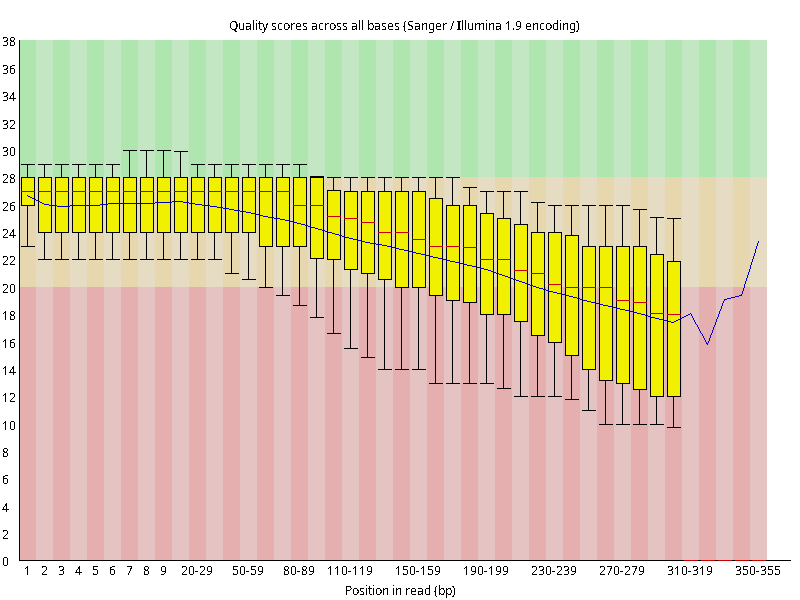
\includegraphics[height=\linewidth, width=\linewidth]{imagens/read\_qc/002.png}
	  \end{minipage}
	  \hspace{.05\linewidth}
	  \begin{minipage}{.45\linewidth}
		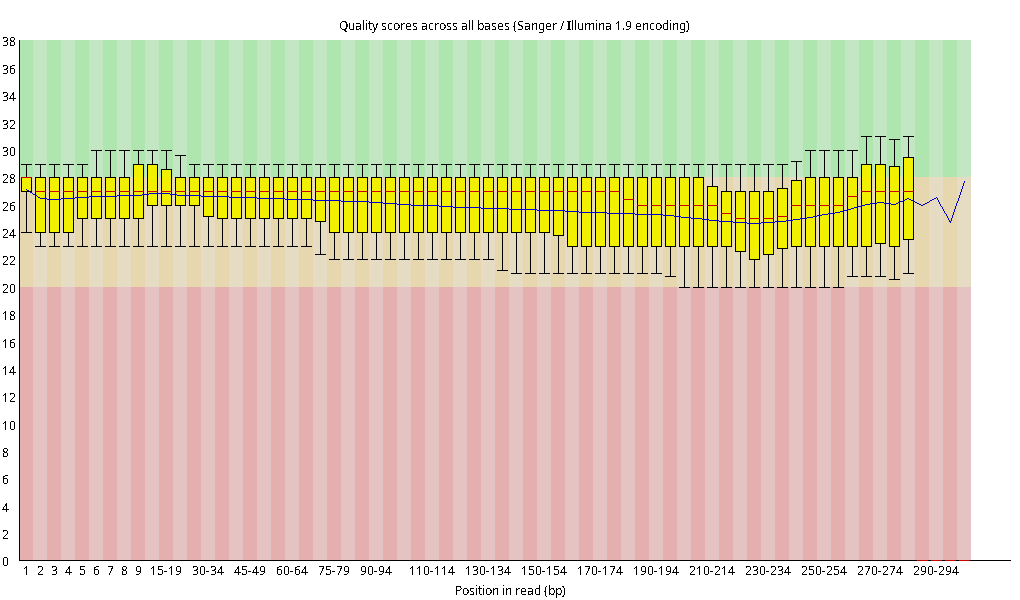
\includegraphics[height=\linewidth ,width=\linewidth]{imagens/read\_qc/002trimmed.png}
	  \end{minipage}
    \begin{small}\textbf{Fonte: O Autor (2022)}\end{small}
\end{figure}
